\chapter{Diagramas binarios sólido--líquido}\label{ch:b2:solid-liquid-diagrams}

El estaño funde a \qty{232}{\degreeCelsius} y el plomo a \qty{327}{\degreeCelsius},
y sin embargo la antigua soldadura de los electricistas, una mezcla de ambos, funde a
\qty{182}{\degreeCelsius}, por debajo de los dos. La sal esparcida en una carretera funde el hielo, pero solo
hasta unos \qty{-21}{\degreeCelsius}; en una noche más fría no sirve de nada.
El cobre y el níquel, en cambio, se mezclan en cualquier proporción incluso en estado
sólido, y sus aleaciones funden en un intervalo de temperaturas comprendido entre las de los
dos metales. Los diagramas de este capítulo dicen, para cada par, qué sólidos
cristalizan a partir de un líquido que se enfría, a qué temperaturas y en qué
cantidades: el saber que hay detrás de cada pieza fundida, de cada unión soldada y de cada
aleación de bajo punto de fusión.

\begin{recall}
\Cref{ch:b2:chemical-potential}: \omterm{def:b2:chemical-potential:chemical-potential}{potencial químico} de un componente en una \omterm{def:b2:chemical-potential:ideal-mixture}{mezcla
ideal}, crioscopia. \Cref{ch:b2:equilibrium-shifts}: la \omterm{def:b2:equilibrium-shifts:variance}{varianza}.
\Cref{ch:b2:liquid-vapour-diagrams}: \omterm{def:b2:liquid-vapour-diagrams:binary-diagram}{diagramas binarios}, rectas de reparto y \omterm{thm:b2:liquid-vapour-diagrams:lever}{regla de la
palanca}. El volumen del primer año: enlace metálico, aleaciones de sustitución e
intersticiales, tipos de cristales.
\end{recall}

\begin{omfigure}
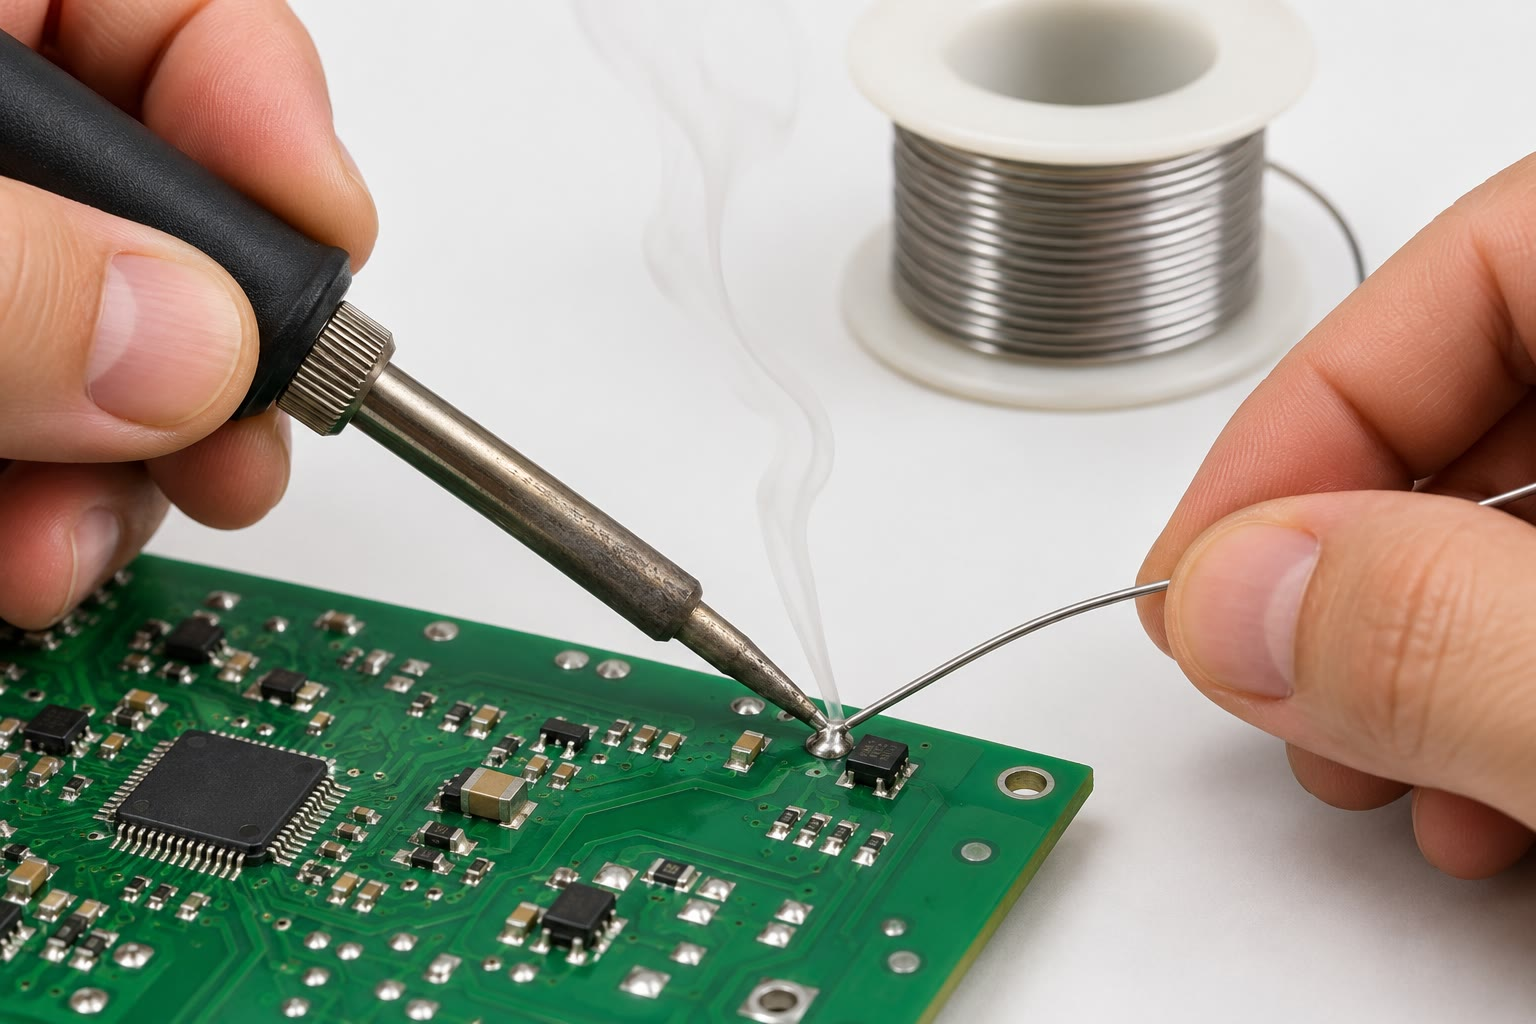
\includegraphics[width=0.6\linewidth]{images/book3/ai/b2-08-soldering.jpg}

{\small Soldadura de un componente en una placa de circuito: el hilo de estaño funde en
contacto con el soldador caliente y la unión solidifica en menos de un segundo cuando se retira
el soldador, porque la aleación funde a una única temperatura, baja.}
\end{omfigure}

\section{Análisis térmico}

\begin{definition}[Análisis térmico]\label{def:b2:solid-liquid-diagrams:cooling-curve}
El \emph{análisis térmico}\index{analisis termico@análisis térmico} determina las temperaturas de
los cambios de estado de una muestra a partir de su temperatura registrada mientras se
calienta o se enfría a velocidad constante. El registro de la temperatura en función del tiempo
durante un enfriamiento lento es una \emph{curva de enfriamiento}\index{curva de enfriamiento}.
\end{definition}

Lejos de cualquier cambio de estado, la muestra se enfría de forma regular. Cuando un sólido empieza a
cristalizar, el calor de cristalización frena el enfriamiento: la curva presenta un
cambio de pendiente, o se detiene durante un tiempo a temperatura constante (una
\textit{meseta}) si la solidificación ocurre a temperatura fija.

\begin{proposition}[Mesetas]\label{prop:b2:solid-liquid-diagrams:plateaus}
A presión fija, una sustancia pura solidifica a temperatura constante, y lo mismo
ocurre con un líquido binario del que cristalizan dos sólidos a la vez. Un líquido binario
del que cristaliza un solo sólido solidifica en un intervalo de temperaturas.
\end{proposition}

\begin{proof}
Fijada la presión, la \omterm{def:b2:equilibrium-shifts:variance}{varianza} es $v = n - r + 1 - \varphi$. Sustancia
pura, líquido + sólido: $v = 1 + 1 - 2 = 0$. Sistema binario, líquido + dos sólidos:
$v = 2 + 1 - 3 = 0$. Sistema binario, líquido + un sólido: $v = 2 + 1 - 2 = 1$: la
temperatura cambia a la vez que la composición del líquido. Una \omterm{def:b2:equilibrium-shifts:variance}{varianza} 0 significa que la
temperatura no puede cambiar mientras están presentes todas las fases: el calor retirado lo
aporta la solidificación, hasta que desaparece una fase.
\end{proof}

\begin{omfigure}
\begin{tikzpicture}[font=\small, x=0.55cm, y=0.05cm]
  \foreach \dx/\name in {0/metal puro, 9/{mezcla, un sólido primero}, 18/mezcla eutéctica} {
    \draw[->] (\dx,0) -- (\dx+7.5,0) node[below left, font=\scriptsize] {$t$};
    \draw[->] (\dx,0) -- (\dx,62) node[above, font=\scriptsize] {$T$};
    \node[font=\scriptsize] at (\dx+3.8,-8) {\name};
  }
  % pure: cool, plateau at 40, cool
  \draw[omDef, thick] (0,58) .. controls (1,48) and (1.6,42) .. (2,40) -- (4.5,40) .. controls (5.2,32) and (6,24) .. (7,20);
  \node[font=\scriptsize, anchor=south] at (3.25,40.5) {meseta};
  % mixture: cool, break at 48, slow fall, plateau at 30, cool
  \draw[omDef, thick] (9,58) .. controls (9.6,53) and (9.9,50) .. (10.2,48)
     .. controls (11,42) and (11.6,35) .. (12.3,30) -- (14.2,30) .. controls (14.9,23) and (15.6,17) .. (16.5,14);
  \node[font=\scriptsize, anchor=west] at (10.4,49.5) {cambio de pendiente};
  \node[font=\scriptsize, anchor=south] at (13.25,30.5) {eutéctico};
  % eutectic: plateau at 30
  \draw[omDef, thick] (18,58) .. controls (19,46) and (19.8,36) .. (20.5,30) -- (24,30) .. controls (24.7,23) and (25.4,17) .. (26.2,14);
  \node[font=\scriptsize, anchor=south] at (22.25,30.5) {meseta};
\end{tikzpicture}

{\small \omterm{def:b2:solid-liquid-diagrams:cooling-curve}{Curvas de enfriamiento}, esquemáticas. Un metal puro solidifica en una meseta. Una
mezcla presenta un cambio de pendiente cuando aparece el primer sólido, luego el enfriamiento
lento de un líquido que solidifica en un intervalo de temperaturas, y luego la
meseta del eutéctico. Un líquido de composición eutéctica solidifica en una
sola meseta, como una sustancia pura.}
\end{omfigure}

\begin{method}[Construir un diagrama a partir de curvas de enfriamiento]\label{met:b2:solid-liquid-diagrams:diagram-from-curves}
\begin{enumerate}
  \item Regístrense \omterm{def:b2:solid-liquid-diagrams:cooling-curve}{curvas de enfriamiento} para una serie de composiciones, componentes
        puros incluidos.
  \item En una gráfica (composición, temperatura), represéntense para cada composición la
        temperatura del primer cambio de pendiente (el inicio de la cristalización) y la de
        cada meseta.
  \item Únanse los puntos de primera cristalización: es el \omterm{def:b2:solid-liquid-diagrams:liquidus}{liquidus}. Únanse
        los finales de la solidificación: el \omterm{def:b2:solid-liquid-diagrams:liquidus}{solidus}. Una meseta hallada a la misma
        temperatura para muchas composiciones es una recta invariante (un eutéctico).
  \item La duración de la meseta eutéctica, máxima en la composición
        eutéctica, permite localizar esa composición.
\end{enumerate}
\end{method}

\section{Miscibilidad total en el sólido}

\begin{definition}[Disolución sólida]\label{def:b2:solid-liquid-diagrams:solid-solution}
Una \emph{disolución sólida}\index{disolucion solida@disolución sólida} es una única fase cristalina de
composición variable, en la que átomos de un componente sustituyen a átomos del
otro en los sitios de la misma red (de sustitución) u ocupan los huecos de
esa red (intersticial).
\end{definition}

El cobre y el níquel tienen la misma estructura cúbica centrada en las caras y átomos de radios
próximos: forman una \omterm{def:b2:solid-liquid-diagrams:solid-solution}{disolución sólida} de sustitución en todas las composiciones.

\begin{definition}[Liquidus y solidus]\label{def:b2:solid-liquid-diagrams:liquidus}
En un diagrama sólido--líquido, el \emph{liquidus}\index{liquidus} es la curva
por encima de la cual todo es líquido; da la composición del líquido en
equilibrio con un sólido. El \emph{solidus}\index{solidus} es la curva por debajo de
la cual todo es sólido; cuando el sólido es una disolución, da la
composición del sólido en equilibrio con el líquido.
\end{definition}

\begin{proposition}[El huso]\label{prop:b2:solid-liquid-diagrams:lens}
Si los dos componentes forman disoluciones ideales en el líquido y en el sólido,
el \omterm{def:b2:solid-liquid-diagrams:liquidus}{liquidus} y el \omterm{def:b2:solid-liquid-diagrams:liquidus}{solidus} unen los dos puntos de fusión y encierran un
dominio bifásico en forma de huso; a cada temperatura las fracciones molares $x_i$ de
cada componente en el líquido y en el sólido están relacionadas por
\[
  \frac{x_i^{\ell}}{x_i^{s}} = \exp\left[-\frac{\Delta_{\text{fus}}H_i}{R}\left(\frac1T - \frac1{T_i^*}\right)\right] .
\]
\end{proposition}

\begin{proof}
El \omterm{def:b2:chemical-potential:chemical-potential}{potencial químico} de $i$ es el mismo en ambas fases, $\mu_i^{*,s} +
RT\ln x_i^s = \mu_i^{*,\ell} + RT\ln x_i^\ell$, luego $RT\ln(x_i^\ell/x_i^s) =
-(\mu_i^{*,\ell} - \mu_i^{*,s}) = -\Delta_{\text{fus}}G_i(T)$ y, con
$\Delta_{\text{fus}}H_i$ constante, $\Delta_{\text{fus}}G_i = \Delta_{\text{fus}}H_i(1 - T/T_i^*)$.
Junto con $x_1 + x_2 = 1$ en cada fase, las dos relaciones fijan las dos
composiciones a cada $T$ (resueltas numéricamente para la figura); que las
curvas resultantes formen un huso se admite.
\end{proof}

\begin{omfigure}
\begin{tikzpicture}
\begin{axis}[omphase, width=0.62\linewidth, height=7cm, ymin=1050, ymax=1480,
  xlabel={$x$ (níquel)}, ylabel={$T$ (\unit{\degreeCelsius})}]
\addplot[omliquidus] table[x=xl, y=T] {figdata/out/bachelor-2-solid-liquid-a.dat};
\addplot[omsolidus] table[x=xs, y=T] {figdata/out/bachelor-2-solid-liquid-a.dat};
\draw[tieline] (axis cs:0.541,1300) -- (axis cs:0.609,1300);
\fill (axis cs:0.58,1300) circle (1.3pt);
\node[font=\scriptsize] at (axis cs:0.25,1400) {líquido};
\node[font=\scriptsize] at (axis cs:0.8,1150) {disolución sólida};
\node[font=\scriptsize, anchor=east] at (axis cs:0.5,1330) {liquidus};
\node[font=\scriptsize, anchor=west] at (axis cs:0.66,1290) {solidus};
\node[font=\scriptsize, anchor=west] at (axis cs:0.03,1080) {\qty{1085}{\degreeCelsius}};
\draw[black!50] (axis cs:0.005,1084) -- (axis cs:0.03,1080);
\node[font=\scriptsize, anchor=south east] at (axis cs:1.0,1456) {\qty{1455}{\degreeCelsius}};
\end{axis}
\end{tikzpicture}

{\small Cobre--níquel, calculado para disoluciones sólida y líquida ideales a partir de los
puntos de fusión y las entalpías de fusión de los dos metales. A
\qty{1300}{\degreeCelsius} una aleación de composición 0.58 se separa en un líquido
de 0.541 y un sólido de 0.609 (recta de reparto discontinua).}
% ledger: tfus:Cu, dfus:Cu, tfus:Ni, dfus:Ni
\end{omfigure}

\begin{method}[Leer un diagrama sólido--líquido]\label{met:b2:solid-liquid-diagrams:read-solid-liquid}
\begin{enumerate}
  \item Recórrase hacia abajo, desde el líquido, la vertical de la composición
        global.
  \item En el \omterm{def:b2:solid-liquid-diagrams:liquidus}{liquidus} aparece el primer sólido; su composición se lee en
        el otro extremo de la recta de reparto (el \omterm{def:b2:solid-liquid-diagrams:liquidus}{solidus}, o un componente puro).
  \item En el dominio bifásico, léanse las dos composiciones en los extremos de la
        recta de reparto y las proporciones con la \omterm{thm:b2:liquid-vapour-diagrams:lever}{regla de la palanca}, en moles con fracciones
        molares y en masa con fracciones másicas.
  \item En una recta invariante horizontal, la temperatura se detiene hasta que desaparece una fase;
        por debajo, léase el nuevo par de fases.
\end{enumerate}
\end{method}

\begin{example}[Una aleación a \qty{1300}{\degreeCelsius}]\label{ex:b2:solid-liquid-diagrams:lever}
Para la aleación de fracción molar de níquel 0.58 a \qty{1300}{\degreeCelsius}, la
fracción de los átomos en el sólido es $(0.58 - 0.541)/(0.609 - 0.541) = 0.57$.
El primer sólido que aparece, hacia \qty{1315}{\degreeCelsius}, es más rico en níquel
que la aleación, y el último líquido, más pobre.
\end{example}

El diagrama describe el equilibrio, que en un sólido es lento: los primeros cristales,
ricos en níquel, se recubren de capas cada vez más pobres en él a medida que el líquido
cambia, y la difusión en el sólido no tiene tiempo de igualarlas. Una pieza fundida
enfriada deprisa está formada por cristales \textit{zonados}, graduados desde el centro hasta el
borde; un calentamiento prolongado por debajo del \omterm{def:b2:solid-liquid-diagrams:liquidus}{solidus} los homogeneiza.

\section{Miscibilidad nula en el sólido: el eutéctico}

Cuando los dos sólidos no se mezclan en absoluto, cada componente cristaliza puro, y
el \omterm{def:b2:solid-liquid-diagrams:liquidus}{liquidus} tiene dos ramas, una por sólido.

\begin{theorem}[Ecuación de Schröder--van Laar]\label{thm:b2:solid-liquid-diagrams:schroder}
Si un componente A cristaliza puro a partir de una mezcla líquida ideal, el \omterm{def:b2:solid-liquid-diagrams:liquidus}{liquidus}
en el que aparece el sólido A viene dado por
\[
  \ln x_A = -\frac{\Delta_{\text{fus}}H_A}{R}\Big(\frac1T - \frac1{T_A^*}\Big),
\]
siendo $x_A$ la fracción molar de A en el líquido, y $T_A^*$ y
$\Delta_{\text{fus}}H_A$ el punto de fusión y la entalpía de fusión de A puro
(tomada como constante).
\end{theorem}

\begin{proof}
En el equilibrio, el \omterm{def:b2:chemical-potential:chemical-potential}{potencial químico} de A sólido puro es igual al de A en el
líquido: $\mu_A^{*,s}(T) = \mu_A^{*,\ell}(T) + RT\ln x_A$. Por tanto, $R\ln x_A =
-\Delta_{\text{fus}}G_A(T)/T$. Por Gibbs--Helmholtz, $d(\Delta_{\text{fus}}G_A/T)/
dT = -\Delta_{\text{fus}}H_A/T^2$; integrando desde $T_A^*$, donde
$\Delta_{\text{fus}}G_A = 0$, hasta $T$ se obtiene $\Delta_{\text{fus}}G_A/T =
\Delta_{\text{fus}}H_A(1/T - 1/T_A^*)$.
\end{proof}

Para una disolución diluida, $\ln x_A = \ln(1 - x_B) \approx -x_B$ y $1/T -
1/T_A^* \approx -\Delta T/T_A^{*2}$: $\Delta T = RT_A^{*2}x_B/\Delta_{\text{fus}}H_A$,
la ley crioscópica del \cref{ch:b2:chemical-potential}. Para el benceno ($T^* =
\qty{278.64}{K}$, $\Delta_{\text{fus}}H = \qty{9.87}{kJ/mol}$, $M =
\qty{78.11}{g/mol}$), la \omterm{def:b2:chemical-potential:colligative}{constante crioscópica} $RT^{*2}M/\Delta_{\text{fus}}H$
resulta ser \qty{5.11}{K.kg/mol}.
% ledger: tfus:benzene, dfus:benzene

\begin{definition}[Eutéctico]\label{def:b2:solid-liquid-diagrams:eutectic}
El \emph{punto eutéctico}\index{punto eutectico@punto eutéctico} de un sistema binario es el
punto en el que el líquido está en equilibrio con dos sólidos a la vez; es la
temperatura más baja a la que existe un líquido en esa parte del diagrama. Un
líquido de la composición eutéctica, y la mezcla fina e íntima de los dos
sólidos en la que solidifica, se llaman \emph{mezcla
eutéctica}\index{mezcla eutectica@mezcla eutéctica}.
\end{definition}

\begin{corollary}[El eutéctico está donde se cortan las ramas del liquidus]\label{cor:b2:solid-liquid-diagrams:eutectic}
Para dos componentes inmiscibles en el sólido e ideales en el líquido, la
temperatura eutéctica $T_E$ y la composición eutéctica son la solución de
$x_A(T_E) + x_B(T_E) = 1$, viniendo dada cada $x$ por la ecuación de Schröder--van Laar
de su propio sólido.
\end{corollary}

\begin{proof}
En el eutéctico el líquido está saturado de ambos sólidos: está sobre ambas
ramas a la vez, con la misma composición leída en A y en B.
\end{proof}

\begin{omfigure}
\begin{tikzpicture}
\begin{axis}[omphase, width=0.62\linewidth, height=6.5cm, ymin=-25, ymax=85,
  xlabel={$x$ (naftaleno)}, ylabel={$T$ (\unit{\degreeCelsius})}]
\addplot[omliquidus] table[x=x, y=T] {figdata/out/bachelor-2-solid-liquid-b-benzene.dat};
\addplot[omliquidus] table[x=x, y=T] {figdata/out/bachelor-2-solid-liquid-b-naphthalene.dat};
\draw[thick] (axis cs:0,-3.55) -- (axis cs:1,-3.55);
\fill (axis cs:0.133,-3.55) circle (1.5pt);
\node[font=\scriptsize, anchor=north] at (axis cs:0.133,-4.5) {E};
\node[font=\scriptsize] at (axis cs:0.45,72) {líquido};
\node[font=\scriptsize, align=center] at (axis cs:0.65,22) {líquido + naftaleno\\ sólido};
\node[font=\scriptsize, anchor=south west] at (axis cs:0.08,45) {líquido + benceno sólido};
\draw[thin] (axis cs:0.12,45) -- (axis cs:0.06,0.8);
\node[font=\scriptsize] at (axis cs:0.55,-15) {benceno sólido + naftaleno sólido};
\end{axis}
\end{tikzpicture}

{\small Benceno--naftaleno, calculado con la ecuación de Schröder--van Laar
para cada sólido. Las dos ramas se cortan en el eutéctico E,
a \qty{-3.5}{\degreeCelsius} y 0.13 de naftaleno, por debajo del cual todo es sólido.}
% ledger: tfus:benzene, dfus:benzene, tfus:naphthalene, dfus:naphthalene
\end{omfigure}

\begin{example}[Enfriamiento de una mezcla de benceno--naftaleno]\label{ex:b2:solid-liquid-diagrams:naphthalene}
Un líquido de fracción molar de naftaleno 0.5 se enfría hasta la rama del naftaleno
del \omterm{def:b2:solid-liquid-diagrams:liquidus}{liquidus}, hacia \qty{46}{\degreeCelsius}, donde empieza a cristalizar naftaleno sólido
puro. El líquido, que pierde naftaleno, desciende por la
rama; a \qty{-3.5}{\degreeCelsius} alcanza el eutéctico, y el resto
solidifica a temperatura constante en la \omterm{def:b2:solid-liquid-diagrams:eutectic}{mezcla eutéctica}. Por la \omterm{thm:b2:liquid-vapour-diagrams:lever}{regla de la palanca},
justo por encima del eutéctico, el naftaleno sólido es $(0.5 - 0.133)/(1 - 0.133) =
42~\%$ de los moles, y el líquido eutéctico, el 58~\%.
\end{example}

\begin{proposition}[Duración de la meseta eutéctica]\label{prop:b2:solid-liquid-diagrams:plateau-length}
Para muestras de la misma masa enfriadas con la misma velocidad de extracción de calor, la
duración de la meseta eutéctica es proporcional a la cantidad de líquido que
alcanza el eutéctico: máxima para la composición eutéctica y nula para los
componentes puros.
\end{proposition}

\begin{proof}
En la meseta la temperatura es constante: el calor retirado, $\Phi\,\Delta t$
a un ritmo constante $\Phi$, es el calor liberado por la solidificación del
líquido eutéctico, $m_E\,\Delta_{\text{fus}}h_E$. Así, $\Delta t = m_E\,\Delta_{\text{fus}}h_E/
\Phi$, proporcional a la masa $m_E$ de líquido eutéctico, que da la \omterm{thm:b2:liquid-vapour-diagrams:lever}{regla
de la palanca}.
\end{proof}

\section{Miscibilidad parcial y compuestos definidos}

La mayoría de los pares de metales no son ni totalmente miscibles ni totalmente inmiscibles en el
sólido: cada uno disuelve un poco del otro. El plomo disuelve hasta un 19~\% de estaño
en masa, y el estaño hasta un 3.4~\% de plomo. El diagrama contiene entonces dos \omterm{def:b2:solid-liquid-diagrams:solid-solution}{disoluciones
sólidas}, (Pb) y (Sn), y un eutéctico entre ellas; la recta eutéctica ya
no llega a los lados del diagrama, sino que se detiene en los límites de las \omterm{def:b2:solid-liquid-diagrams:solid-solution}{disoluciones
sólidas}.

\begin{omfigure}
\begin{tikzpicture}[font=\small, x=0.075cm, y=0.022cm]
  \draw[->] (0,0) -- (106,0) node[right] {\% Sn (masa)};
  \draw[->] (0,0) -- (0,360) node[above] {$T$ (\unit{\degreeCelsius})};
  \foreach \t in {100,200,300} \draw (0,\t) -- (-1.5,\t) node[left, font=\scriptsize] {\t};
  \foreach \w in {0,20,40,60,80,100} \draw (\w,0) -- (\w,-5) node[below, font=\scriptsize] {\w};
  % invariant points (NIST): Pb 327.5, Sn 231.9, eutectic 182.2 at 62.13; limits 18.91 and 96.59
  \draw[omliquidus] (0,327.5) .. controls (25,290) and (45,235) .. (62.13,182.2);
  \draw[omliquidus] (100,231.9) .. controls (85,215) and (72,200) .. (62.13,182.2);
  \draw[omsolidus] (0,327.5) .. controls (8,280) and (14,220) .. (18.91,182.2);
  \draw[omsolidus] (100,231.9) .. controls (98.5,215) and (97.5,200) .. (96.59,182.2);
  \draw[thick] (18.91,182.2) -- (96.59,182.2);
  \draw[omsolidus, densely dashed] (18.91,182.2) .. controls (12,120) and (6,60) .. (3,20);
  \draw[omsolidus, densely dashed] (96.59,182.2) .. controls (98.5,120) and (99.3,60) .. (99.6,20);
  \fill (62.13,182.2) circle (1.5pt);
  \fill (18.91,182.2) circle (1.2pt); \fill (96.59,182.2) circle (1.2pt);
  \node[anchor=south, font=\scriptsize] at (62.13,186) {E};
  \node[font=\scriptsize] at (55,300) {líquido};
  \node[font=\scriptsize] at (6,150) {(Pb)};
  \node[font=\scriptsize] at (103,140) {(Sn)};
  \node[font=\scriptsize] at (28,235) {L + (Pb)};
  \node[font=\scriptsize] at (84,192) {L + (Sn)};
  \node[font=\scriptsize] at (55,100) {(Pb) + (Sn)};
  % cooling path at 40 %
  \draw[->, omProp, thick] (40,340) -- (40,30);
  \node[font=\scriptsize, omProp, anchor=south] at (40,342) {40~\%};
  \node[font=\scriptsize, anchor=north east] at (16.6,179) {18.9};
  \node[font=\scriptsize, anchor=north] at (62.13,178) {62.1};
  \node[font=\scriptsize, anchor=north east] at (95.8,178) {96.6};
  \node[font=\scriptsize, anchor=west] at (101,182.2) {\qty{182.2}{\degreeCelsius}};
\end{tikzpicture}

{\small El diagrama plomo--estaño, trazado a partir de sus puntos invariantes: puntos
de fusión del plomo (\qty{327.5}{\degreeCelsius}) y del estaño (\qty{231.9}{\degreeCelsius}),
eutéctico E a \qty{182.2}{\degreeCelsius} y 62.1~\% de estaño, límites de las \omterm{def:b2:solid-liquid-diagrams:solid-solution}{disoluciones
sólidas} a la temperatura eutéctica (18.9~\% y 96.6~\% de estaño). Las curvas
entre esos puntos, y los límites de solubilidad discontinuos por debajo del eutéctico,
están trazados de forma esquemática. Flecha: el enfriamiento de una soldadura al 40~\%.}
% ledger: eut:Pb-Sn.T, eut:Pb-Sn.wL, eut:Pb-Sn.wPb, eut:Pb-Sn.wSn, tfus:Pb, tfus:Sn
\end{omfigure}

Una soldadura con un 40~\% de estaño empieza a solidificar en el \omterm{def:b2:solid-liquid-diagrams:liquidus}{liquidus} depositando cristales de
la disolución rica en plomo (Pb); el líquido se enriquece en estaño hasta que, a
\qty{182.2}{\degreeCelsius}, alcanza la composición eutéctica y solidifica en
una mezcla fina de láminas de (Pb) y (Sn), alrededor de los cristales primarios.

\begin{omfigure}
\begin{tikzpicture}[font=\small]
  \begin{scope}
    \clip (0,0) circle (2.2);
    \fill[gray!20] (-2.3,-2.3) rectangle (2.3,2.3);
    \foreach \k in {-24,...,24} \draw[gray!65, line width=1.1pt] (-2.4+0.2*\k,-2.4) -- ++(55:6);
    \foreach \cx/\cy/\r/\a in {-0.9/0.8/0.55/10, 0.7/1.0/0.45/40, 0.2/-0.6/0.6/-20, -1.1/-0.9/0.4/70, 1.3/-0.3/0.35/5} {
      \fill[omDef!35, draw=omDef, rotate around={\a:(\cx,\cy)}] (\cx,\cy) ellipse ({\r} and {0.7*\r});
    }
  \end{scope}
  \draw[thick] (0,0) circle (2.2);
  \draw[<-, omProp, thick] (0.7,1.0) -- (3.0,1.6) node[right, text=black] {cristal primario de (Pb)};
  \draw[<-, omProp, thick] (1.6,0.9) -- (3.0,0.5) node[right, text=black, align=left] {eutéctico: láminas\\ alternas de (Pb) y (Sn)};
\end{tikzpicture}

{\small La microestructura de una soldadura con un 40~\% de estaño tras un enfriamiento lento, esquemática:
cristales primarios de (Pb), formados entre el \omterm{def:b2:solid-liquid-diagrams:liquidus}{liquidus} y el eutéctico, en una
matriz de eutéctico formada por finas láminas alternas de las dos \omterm{def:b2:solid-liquid-diagrams:solid-solution}{disoluciones
sólidas}.}
\end{omfigure}

\begin{definition}[Compuesto definido]\label{def:b2:solid-liquid-diagrams:defined-compound}
Un \emph{compuesto definido}\index{compuesto definido} es un sólido de
composición fija $\mathrm{A}_a\mathrm{B}_b$ formado por los dos componentes. Presenta
\emph{fusión congruente}\index{fusion congruente@fusión congruente} cuando funde dando un líquido de
su misma composición: el \omterm{def:b2:solid-liquid-diagrams:liquidus}{liquidus} tiene entonces un máximo en esa composición.
\end{definition}

Un compuesto de \omterm{def:b2:solid-liquid-diagrams:defined-compound}{fusión congruente} divide el diagrama en dos: cada mitad, A con
$\mathrm{A}_a\mathrm{B}_b$ y $\mathrm{A}_a\mathrm{B}_b$ con B, es un diagrama
propio, con su propio eutéctico. La composición del máximo, leída en fracción
molar, da la fórmula del compuesto.

\begin{omfigure}
\begin{tikzpicture}[font=\small, x=6cm, y=0.05cm]
  \draw[->] (0,0) -- (1.06,0) node[right] {$x_{\mathrm B}$};
  \draw[->] (0,0) -- (0,95) node[above] {$T$};
  \node[below, font=\scriptsize] at (0,0) {A}; \node[below, font=\scriptsize] at (1,0) {B};
  \node[below, font=\scriptsize] at (0.667,0) {$\tfrac23$};
  \draw[omliquidus] (0,70) .. controls (0.12,58) and (0.25,45) .. (0.35,35);
  \draw[omliquidus] (0.35,35) .. controls (0.45,62) and (0.58,79) .. (0.667,80);
  \draw[omliquidus] (0.667,80) .. controls (0.75,79) and (0.8,68) .. (0.85,50);
  \draw[omliquidus] (0.85,50) .. controls (0.9,56) and (0.95,62) .. (1,65);
  \draw[thick] (0,35) -- (0.667,35); \draw[thick] (0.667,50) -- (1,50);
  \draw[thick] (0.667,0) -- (0.667,80);
  \fill (0.35,35) circle[radius=1.5pt]; \fill (0.85,50) circle[radius=1.5pt];
  \fill (0.667,80) circle[radius=1.5pt];
  \node[anchor=north, font=\scriptsize] at (0.35,34) {E$_1$};
  \node[anchor=north, font=\scriptsize] at (0.85,49) {E$_2$};
  \node[anchor=south, font=\scriptsize] at (0.667,81) {fusión de $\mathrm{AB_2}$};
  \node[font=\scriptsize] at (0.35,80) {líquido};
  \node[font=\scriptsize, align=center] at (0.33,15) {A +\\ $\mathrm{AB_2}$};
  \node[font=\scriptsize, align=center] at (0.84,25) {$\mathrm{AB_2}$\\ + B};
\end{tikzpicture}

{\small Diagrama esquemático con un \omterm{def:b2:solid-liquid-diagrams:defined-compound}{compuesto definido} $\mathrm{AB_2}$ (recta vertical
en $x_{\mathrm B} = 2/3$) de \omterm{def:b2:solid-liquid-diagrams:defined-compound}{fusión congruente} en el máximo del
\omterm{def:b2:solid-liquid-diagrams:liquidus}{liquidus}. El diagrama son dos diagramas eutécticos simples uno junto a otro, con
los eutécticos E$_1$ y E$_2$.}
\end{omfigure}

\section{Aplicaciones}

\paragraph{Soldaduras y aleaciones de bajo punto de fusión.} Una soldadura debe fundir por debajo de las piezas
que une y solidificar deprisa, sin intervalo pastoso: la composición eutéctica es
la elección natural. El eutéctico estaño--plomo funde a \qty{182.2}{\degreeCelsius};
como el plomo es tóxico, la electrónica usa hoy soldaduras sin plomo, entre ellas el
eutéctico bismuto--estaño, que funde a \qty{138.8}{\degreeCelsius} y contiene un
57~\% de bismuto en masa.
% ledger: eut:Pb-Sn.T, eut:Bi-Sn.T, eut:Bi-Sn.wL

\paragraph{Deshielo.} El hielo y la sal forman un eutéctico: el eutéctico hielo--dihidrato
de la sal se sitúa a \qty{252}{K} (\qty{-21}{\degreeCelsius}) y 23.3~\% de cloruro
de sodio en masa. Por encima de esa temperatura, la sal en contacto con el hielo forma una
salmuera cuyo punto de congelación está por debajo de la temperatura de la carretera, y el hielo
se funde; por debajo, no puede existir ningún líquido, y la sal es inútil.
% ledger: eut:NaCl-water.T, eut:NaCl-water.w

\paragraph{Cristalización.} El diagrama de una sal y el agua se lee como cualquier
otro: enfriar una disolución saturada caliente atraviesa la curva de solubilidad (el
\omterm{def:b2:solid-liquid-diagrams:liquidus}{liquidus} de la sal), y se depositan cristales puros de la sal mientras que las
impurezas, demasiado diluidas para alcanzar su propio \omterm{def:b2:solid-liquid-diagrams:liquidus}{liquidus}, quedan en las aguas madres.
Es la purificación por recristalización del volumen del primer año, vista sobre un
diagrama.

\begin{omfigure}
\begin{tikzpicture}
\begin{axis}[omphase, width=0.62\linewidth, height=6cm, xmin=0, xmax=100,
  ymin=90, ymax=285, xlabel={\% Bi (masa)}, ylabel={$T$ (\unit{\degreeCelsius})}]
\addplot[omliquidus] table[x=w, y=T] {figdata/out/bachelor-2-solid-liquid-d-Sn.dat};
\addplot[omliquidus] table[x=w, y=T] {figdata/out/bachelor-2-solid-liquid-d-Bi.dat};
\draw[densely dashed] (axis cs:0,119.5) -- (axis cs:100,119.5);
\fill[omThm] (axis cs:56.97,138.8) circle (2pt);
\node[font=\scriptsize, omThm, anchor=west] at (axis cs:64,129) {eutéctico evaluado};
\draw[omThm, thin] (axis cs:64,129) -- (axis cs:57.8,137.6);
\node[font=\scriptsize, anchor=north] at (axis cs:52,118) {modelo ideal};
\node[font=\scriptsize] at (axis cs:50,250) {líquido};
\end{axis}
\end{tikzpicture}

{\small Bismuto--estaño: el \omterm{def:b2:solid-liquid-diagrams:liquidus}{liquidus} previsto para sólidos puros y un líquido
ideal (Schröder--van Laar, azul) tiene su eutéctico cerca de
\qty{120}{\degreeCelsius}; el eutéctico evaluado (punto rojo) está a
\qty{138.8}{\degreeCelsius} y 57~\% de bismuto.}
% ledger: tfus:Sn, dfus:Sn, tfus:Bi, dfus:Bi, eut:Bi-Sn.T, eut:Bi-Sn.wL
\end{omfigure}

\section{Ejercicios}

\begin{exercise}[$\star$]\label{exo:b2:solid-liquid-diagrams:1}
En el diagrama cobre--níquel, dense las fases presentes a
\qty{1300}{\degreeCelsius} para fracciones molares de níquel de 0.40, 0.58 y 0.70.
\end{exercise}

\begin{exercise}[$\star$]\label{exo:b2:solid-liquid-diagrams:2}
Se mantienen \qty{2.00}{mol} de una aleación cobre--níquel de fracción molar de níquel 0.58
a \qty{1300}{\degreeCelsius}. Calcúlense las cantidades de sólido y de líquido y la
cantidad de níquel en cada uno.
\end{exercise}

\begin{exercise}[$\star$]\label{exo:b2:solid-liquid-diagrams:3}
Calcúlese la \omterm{def:b2:equilibrium-shifts:variance}{varianza} a presión fija (a) de un metal puro mientras solidifica;
(b) de una aleación cobre--níquel mientras solidifica; (c) de un líquido plomo--estaño en la
recta eutéctica.
\end{exercise}

\begin{exercise}[$\star$]\label{exo:b2:solid-liquid-diagrams:4}
Esbócese la \omterm{def:b2:solid-liquid-diagrams:cooling-curve}{curva de enfriamiento} del estaño puro de \qty{300}{\degreeCelsius} a
\qty{100}{\degreeCelsius} y explíquese por qué la temperatura se detiene a
\qty{232}{\degreeCelsius}.
\end{exercise}

\begin{exercise}[$\star\star$]\label{exo:b2:solid-liquid-diagrams:5}
Con los datos del capítulo (benceno \qty{278.64}{K}, \qty{9.87}{kJ/mol};
naftaleno \qty{353.2}{K}, \qty{19.1}{kJ/mol}), compruébese que a
\qty{269.6}{K} las dos fracciones molares de Schröder--van Laar suman 1, y dese
la composición eutéctica.
\end{exercise}

\begin{exercise}[$\star\star$]\label{exo:b2:solid-liquid-diagrams:6}
Descríbase el enfriamiento de una aleación plomo--estaño con un 30~\% de estaño en masa, desde el líquido
hasta la temperatura ambiente, y calcúlese la fracción másica de eutéctico que contiene.
\end{exercise}

\begin{exercise}[$\star\star$]\label{exo:b2:solid-liquid-diagrams:7}
¿Qué masa de cloruro de sodio por kilogramo de agua contiene la salmuera
eutéctica? ¿Por qué es inútil salar una carretera a \qty{-25}{\degreeCelsius}?
\end{exercise}

\begin{exercise}[$\star\star$]\label{exo:b2:solid-liquid-diagrams:8}
En el diagrama esquemático con el compuesto $\mathrm{AB_2}$, descríbase el
enfriamiento de líquidos de $x_{\mathrm B} = 0.5$ y $x_{\mathrm B} = 0.9$: primer
sólido, eutéctico alcanzado, sólidos al final.
\end{exercise}

\begin{exercise}[$\star\star$]\label{exo:b2:solid-liquid-diagrams:9}
En la fusión por zonas, se hace pasar lentamente una zona fundida a lo largo de una barra. Cerca del níquel puro,
la razón de las fracciones molares de cobre en el sólido y en el líquido en
equilibrio es de 0.78 aproximadamente. Explíquese por qué el cobre es arrastrado por la
zona fundida, y por qué hacen falta varias pasadas.
\end{exercise}

\begin{exercise}[$\star\star\star$]\label{exo:b2:solid-liquid-diagrams:10}
Dedúzcase la ecuación de Schröder--van Laar y demuéstrese después que para un líquido diluido
se reduce a $\Delta T = K_f\,b$, con $K_f = RT^{*2}M_A/\Delta_{\text{fus}}H_A$
y $b$ la molalidad del soluto; calcúlese $K_f$ para el benceno.
\end{exercise}

\begin{exercise}[$\star\star\star$]\label{exo:b2:solid-liquid-diagrams:11}
El diagrama magnesio--plomo presenta un máximo del \omterm{def:b2:solid-liquid-diagrams:liquidus}{liquidus} a un 19.0~\% de magnesio en
masa. Hállese la fórmula del compuesto.
\end{exercise}

\begin{exercise}[$\star\star\star$]\label{exo:b2:solid-liquid-diagrams:12}
Se enfrían en las mismas condiciones masas iguales de aleaciones plomo--estaño. La
aleación eutéctica presenta una meseta de \qty{300}{s}; una aleación desconocida, una de
\qty{120}{s}. Hállense las dos composiciones posibles de la desconocida, y dígase cómo
distinguirlas.
\end{exercise}

\section{Problema: la soldadura}

\begin{problem}[{Problema de fin de semana --- el diagrama plomo--estaño a partir de sus puntos
invariantes, la solidificación de una soldadura al 40~\% con la regla de la palanca, una soldadura
sin plomo de bismuto--estaño prevista por el modelo de líquido ideal y la elección de una
soldadura}]
\label{pb:b2:solid-liquid-diagrams:1}
Datos (NIST, equilibrios invariantes calculados): eutéctico plomo--estaño a
\qty{182.2}{\degreeCelsius}, líquido de 62.13~\% de estaño en masa, en equilibrio con
(Pb) de 18.91~\% y (Sn) de 96.59~\% de estaño; eutéctico bismuto--estaño a
\qty{138.8}{\degreeCelsius}, líquido de 56.97~\% de bismuto. Puntos de fusión y
entalpías de fusión: plomo \qty{600.6}{K}, \qty{4.77}{kJ/mol}; estaño
\qty{505.1}{K}, \qty{7.03}{kJ/mol}; bismuto \qty{544.6}{K}, \qty{11.30}{kJ/mol}.
Masas molares (\unit{g/mol}): Pb 207.2, Sn 118.71, Bi 208.98.
% ledger: eut:Pb-Sn.T, eut:Pb-Sn.wL, eut:Pb-Sn.wPb, eut:Pb-Sn.wSn, eut:Bi-Sn.T, eut:Bi-Sn.wL, tfus:Pb, dfus:Pb, tfus:Sn, dfus:Sn, tfus:Bi, dfus:Bi, aw:Pb, aw:Sn, aw:Bi

\medskip
\noindent\textbf{Parte I --- El diagrama plomo--estaño.}
\begin{enumerate}
  \item Conviértanse a grados Celsius los puntos de fusión del plomo y del estaño.
  \item Conviértase la composición eutéctica en fracción molar de estaño.
  \item Sitúense en una gráfica (\% en masa de Sn, $T$) los puntos de fusión, el eutéctico y
        los dos extremos de la recta eutéctica.
  \item Trácese el diagrama y nómbrense sus seis dominios.
  \item Escríbase la transformación eutéctica en el enfriamiento.
  \item Calcúlese la \omterm{def:b2:equilibrium-shifts:variance}{varianza} en la recta eutéctica a presión fija.
\end{enumerate}

\medskip
\noindent\textbf{Parte II --- Enfriamiento de una soldadura al 40~\%.}
\begin{enumerate}[resume]
  \item ¿Qué sólido aparece primero, y por qué no es plomo puro?
  \item ¿Cómo cambia la composición del líquido durante el enfriamiento hasta
        el eutéctico?
  \item Justo por encima de \qty{182.2}{\degreeCelsius}: ¿qué fases, y de qué
        composiciones?
  \item Calcúlense sus fracciones másicas.
  \item Justo por debajo: ¿qué fases, de qué composiciones y en qué fracciones
        másicas?
  \item ¿Qué fracción de la aleación está formada por constituyente eutéctico, y qué
        fracción por cristales primarios de (Pb)?
  \item Esbócese la \omterm{def:b2:solid-liquid-diagrams:cooling-curve}{curva de enfriamiento} y compárese su meseta con la de la
        aleación eutéctica.
\end{enumerate}

\medskip
\noindent\textbf{Parte III --- Una soldadura sin plomo según el modelo de líquido ideal.}
\begin{enumerate}[resume]
  \item Escríbase la ecuación de Schröder--van Laar para el \omterm{def:b2:solid-liquid-diagrams:liquidus}{liquidus} del estaño.
  \item Escríbase para el \omterm{def:b2:solid-liquid-diagrams:liquidus}{liquidus} del bismuto.
  \item Escríbase la condición que define el eutéctico.
  \item Calcúlese la suma de las dos fracciones molares a \qty{110}{\degreeCelsius},
        \qty{120}{\degreeCelsius} y \qty{130}{\degreeCelsius}, y hállese la
        temperatura eutéctica del modelo con una precisión de un grado.
  \item Dese la composición eutéctica del modelo, en fracción molar y en fracción
        másica de bismuto.
  \item Compárese con el eutéctico evaluado.
  \item El estaño disuelve hasta un 21~\% de bismuto en estado sólido. Explíquese cómo esto
        hace el eutéctico real más caliente que el del modelo.
\end{enumerate}

\medskip
\noindent\textbf{Parte IV --- La elección de una soldadura.}
\begin{enumerate}[resume]
  \item ¿Por qué se prefiere una composición eutéctica para una soldadura?
  \item Dese una razón para sustituir el plomo en las soldaduras.
  \item ¿Qué ofrece el bajo punto de fusión del eutéctico bismuto--estaño, y
        qué podría costar?
  \item Calcúlense las masas de bismuto y de estaño en \qty{1.00}{kg} de
        soldadura eutéctica bismuto--estaño.
  \item Indíquese la temperatura eutéctica del bismuto--estaño prevista por el
        modelo de líquido ideal.
\end{enumerate}
\end{problem}
